\section{Determinants of Order 2} \label{sec 4.1}

In this section, we define the determinant of a \(2 \X 2\) matrix and investigate its \emph{geometric significance} in terms of \emph{area and orientation}.

\begin{definition} \label{def 4.1}
If
\[
    A = \begin{pmatrix} a & b \\ c & d \end{pmatrix}
\]
is a \(2 \X 2\) matrix with entries from a field \(F\), then we define the \textbf{determinant} of \(A\), denoted \(\det(A)\) or \(\abs{A}\), to be the scalar \(ad - be\).
\end{definition}

\begin{example} \label{example 4.1.1}
For the matrices
\[
    A = \left(\begin{array}{ll} 1 & 2 \\ 3 & 4 \end{array}\right)
    \text{ and }
    B = \left(\begin{array}{ll} 3 & 2 \\ 6 & 4 \end{array}\right)
\]
in \(M_{2 \X 2}(\SET{R})\), we have
\[
    \det(A) = 1 \cdot 4 - 2 \cdot 3 = -2
    \text{ and }
    \det(B) = 3 \cdot 4 - 2 \cdot 6 = 0.
\]
\end{example}

\begin{remark} \label{remark 4.1.1}
For the matrices \(A\) and \(B\) in \EXAMPLE{4.1.1}, we have
\[
  A + B = \left(\begin{array}{ll} 4 & 4 \\ 9 & 8 \end{array}\right)
\]
and so
\[
    \det(A + B) = 4 \cdot 8 - 4 \cdot 9 = -4.
\]
Since \(\det(A + B) \ne \det(A) + \det(B)\), the function \(\det: M_{2 \X 2}(\SET{R}) \to \SET{R}\) is \emph{not} a linear transformation.
\end{remark}

\begin{theorem} \label{thm 4.1}
The function \(\det: M_{2 \X 2}(F) \to F\) is a \emph{linear} function \emph{of each row} of a \(2 \X 2\) matrix \emph{when the other row is held fixed}.
That is, if \(u, v\), and \(w\) are in \(F^2\) and \(k\) is a scalar, then
(we can represent \(\begin{pmatrix} u + kv \\ w \end{pmatrix}\), \(\begin{pmatrix} u \\ w \end{pmatrix}\) and so on as \(2 \X 2\) matrices, and)
\[
    \det\left(\begin{array}{c} u + kv \\ w \end{array}\right)
    = \det\left(\begin{array}{c} u \\ w \end{array}\right)
    + k \det\left(\begin{array}{c} v \\ w \end{array}\right)
\]
and
\[
    \det\left(\begin{array}{c} w \\ u + k v \end{array}\right)
    = \det\left(\begin{array}{l} w \\ u \end{array}\right)
    + k \det\left(\begin{array}{l} w \\ v \end{array}\right).
\]
\end{theorem}

\begin{proof}
Let \(u = (a_1, a_2), v = (b_1, b_2)\), and \(w = (c_1, c_2)\) be in \(F^2\) and \(k\) be a scalar.
Then
\begin{align*}
    \det\begin{pmatrix} u + kv \\ w \end{pmatrix}
        & = \det\begin{pmatrix} a_1 + k b_1 & a_2 + k b_2 \\ c_1 & c_2 \end{pmatrix} \\
        & = (a_1 + k b_1) c_2 - (a_2 + k b_2) c_1 & \text{by \DEF{3.1}} \\
        & \RED{ = } a_1 c_2 - a_2 c_1 + k(b_1 c_2 - b_2 c_1) \\
        & = \det\begin{pmatrix} a_1 & a_2 \\ c_1 & c_2 \end{pmatrix} + k \det\begin{pmatrix} b_1 & b_2 \\ c_1 & c_2 \end{pmatrix} & \text{again by \DEF{3.1}} \\
        & = \det\begin{pmatrix} u \\ w \end{pmatrix} + k \det\begin{pmatrix} v \\ w \end{pmatrix}.
\end{align*}
A similar calculation show that
\[
    \det\left(\begin{array}{c} w \\ u + k v \end{array}\right)
    = \det\left(\begin{array}{l} w \\ u \end{array}\right)
    + k \det\left(\begin{array}{l} w \\ v \end{array}\right).
\]
\end{proof}

\begin{note}
For the \(2 \X 2\) matrices \(A\) and \(B\) in \EXAMPLE{4.1.1}, it is easily checked that \(A\) is invertible but \(B\) is not. Note that \(\det(A) \ne 0\) but \(\det(B) = 0\).
We now show that this property is \emph{true in general}.
\end{note}

\begin{theorem} \label{thm 4.2}
Let \(A \in M_{2 \X 2}(F)\).
Then the determinant of \(A\) is nonzero if and only if \(A\) is invertible.
Moreover, if \(A\) is invertible, then
\[
    A^{-1} = \frac{1}{\det(A)}\left(\begin{array}{rr}
                A_{22} & -A_{12} \\
                -A_{21} & A_{11}
            \end{array}\right).
\]
\end{theorem}

\begin{proof}
If \(\det(A) \ne 0\), then we can define a matrix
\[
    M = \frac{1}{\det(A)}\left(\begin{array}{rr}
            A_{22} & -A_{12} \\
            -A_{21} & A_{11}
        \end{array}\right).
\]
A straightforward calculation shows that \(AM = MA = I\), and so \(A\) is invertible and \(M = A^{-1}\).

Conversely, suppose that \(A\) is invertible.
By \RMK{3.2.1} shows that the rank of
\[
    A = \begin{pmatrix} A_{11} & A_{12} \\ A_{21} & A_{22} \end{pmatrix}
\]
must be \(2\).
Hence it's impossible that both \(A_{11}\) and \(A_{21}\) are zero, hence \(A_{11} \ne 0\) or \(A_{21} \ne 0\).
\begin{itemize}
    \item If \(A_{11} \ne 0\), add \(-\frac{A_{21}}{A_{11}}\) times row \(1\) of \(A\) to row \(2\) to obtain the matrix
    \[
        \begin{pmatrix}
            A_{11} & A_{12} \\
            0 & A_{22} - \frac{A_{12}A_{21}}{A_{11}}.
        \end{pmatrix}.
    \]
    Because e.r.o.s are rank-preserving by \CORO{3.4.1}, it follows that the second row of this matrix cannot be zero row.
    That is,
    \[
        A_{22} - \frac{A_{12}A_{21}}{A_{11}} \ne 0.
    \]
    In particular, \(A_{11} A_{22} - A_{12}A_{21} \ne 0\);
    that is, \(\det(A) \ne 0\).
    
    \item On the other hand, if \(A_{21} \ne 0\), we see that \(\det(A) \ne 0\) by adding \(-\frac{A_{11}}{A_{21}}\) times row \(2\) of \(A\) to row \(1\) and applying a similar argument.
\end{itemize}
Thus, in either case, \(\det(A) \ne 0\).
\end{proof}

\begin{remark} \label{remark 4.1.2}
In \SEC{4.2} and \SEC{4.3}, we \emph{extend the definition} of the determinant to \(n \X n\) matrices and show that \THM{4.2} remains true in this more general context.
In the remainder of this section, which can be omitted if desired, we explore the geometric significance of the determinant of a \(2 \X 2\) matrix.
In particular, we show the importance of the \emph{sign} of the value of the determinant in the study of (geometric) orientation.
\end{remark}

\subsection{The Area of a Parallelogram}

\begin{additional definition} \label{adef 4.1}
By the \textbf{angle} between two vectors in \(\SET{R}^2\), we mean the angle with measure \(\theta\) (\(0 \le \theta < \pi\))
that is formed by the vectors \emph{having the same magnitude and direction} as the given vectors \emph{but emanating from the origin}. (See Figure 4.1.)

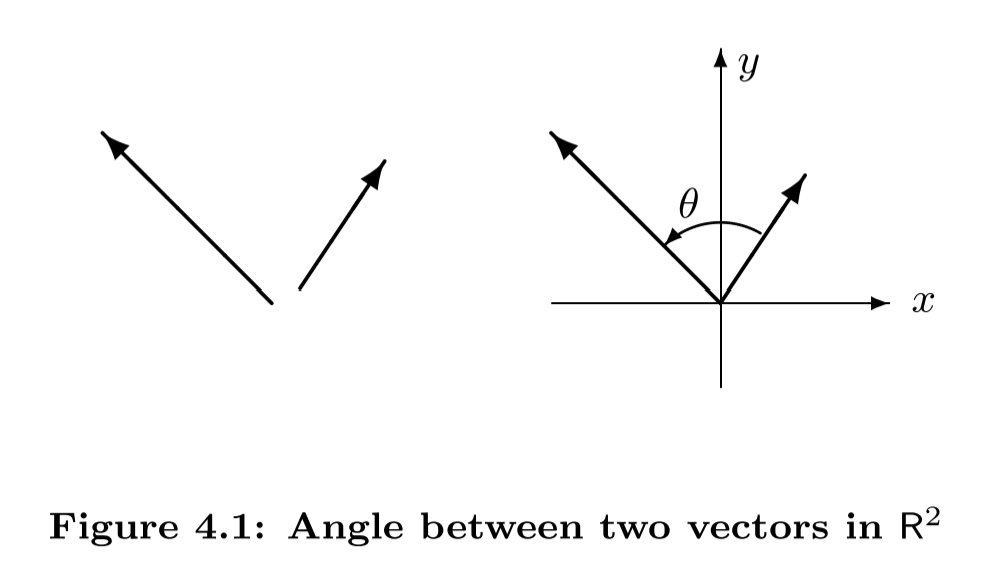
\includegraphics[width=12cm]{images/figure-4-1.png}

If \(\beta = \{ u, v \}\) is an ordered basis for \(\SET{R}^2\), we define the \textbf{orientation} of \(\beta\) to be the \emph{real number}
\[
    \mathcal{O} \begin{pmatrix} u \\ v \end{pmatrix}
    = \frac {\det\begin{pmatrix} u \\ v \end{pmatrix}} {\left| \det\begin{pmatrix} u \\ v \end{pmatrix} \right| }.
\]
(The denominator of this fraction is nonzero by \THM{4.2}.)
Clearly,
\[
    \mathcal{O} \begin{pmatrix} u \\ v \end{pmatrix} = \pm 1.
\]
\end{additional definition}

\begin{additional definition} \label{adef 4.2}
Notice that
\[
    \mathcal{O} \begin{pmatrix} e_1 \\ e_2 \end{pmatrix} = 1.
    \text{ and }
    \mathcal{O} \begin{pmatrix} e_1 \\ \RED{-e_2} \end{pmatrix} = -1.
\]
Recall that a coordinate system \(\{ u, v \}\) is called \textbf{right-handed} if \(u\) can be \emph{rotated in a counterclockwise} direction through an angle \(\theta\) \((0 < \theta < \pi\))to coincide with \(v\).
Otherwise \(\{ u, v \}\) is called a \textbf{left-handed system}.
(See Figure 4.2.)

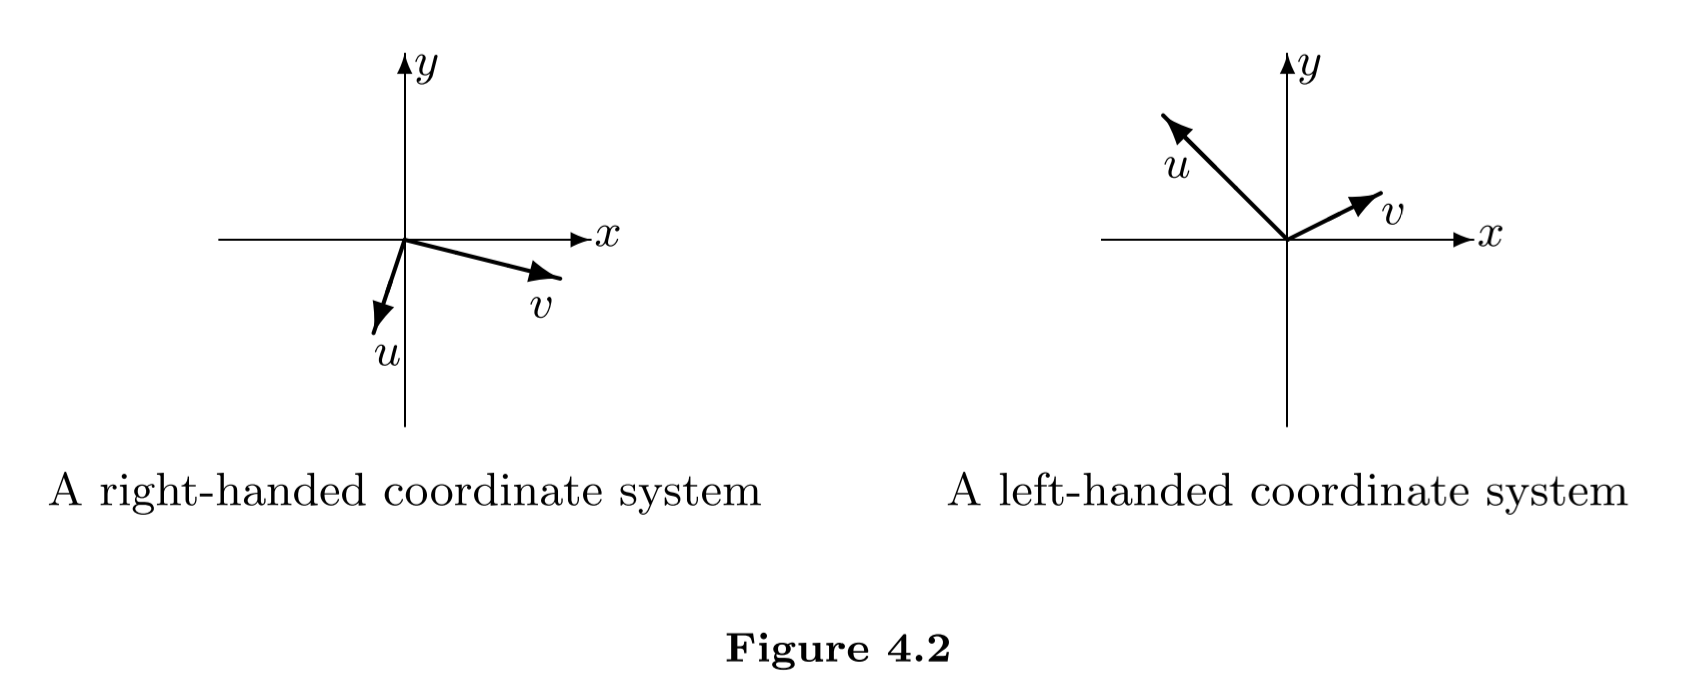
\includegraphics[width=16cm]{images/figure-4-2.png}

In general (see \EXEC{4.1.13}),
\[
    \mathcal{O} \begin{pmatrix} u \\ v \end{pmatrix} = 1.
\]
if and only if the ordered basis \(\{ u, v \}\) forms a right-banded coordinate system.
\end{additional definition}

\begin{remark} \label{remark 4.1.3}
For convenience, we also define
\[
    \mathcal{O} \begin{pmatrix} u \\ v \end{pmatrix} = 1.
\]
if \(\{ u, v \}\) is linearly \textbf{dependent}.
\end{remark}

Any ordered set \(\{ u, v \}\) in \(\SET{R}^2\) determines a parallelogram in the following manner.
Regarding \(u\) and \(v\) as arrows emanating from the origin of \(\SET{R}^2\), we call the \textbf{parallelogram} having \(u\) and \(v\) as \emph{adjacent sides} the \textbf{parallelogram
determined by \(u\) and \(v\)}.
(See Figure 4.3.)

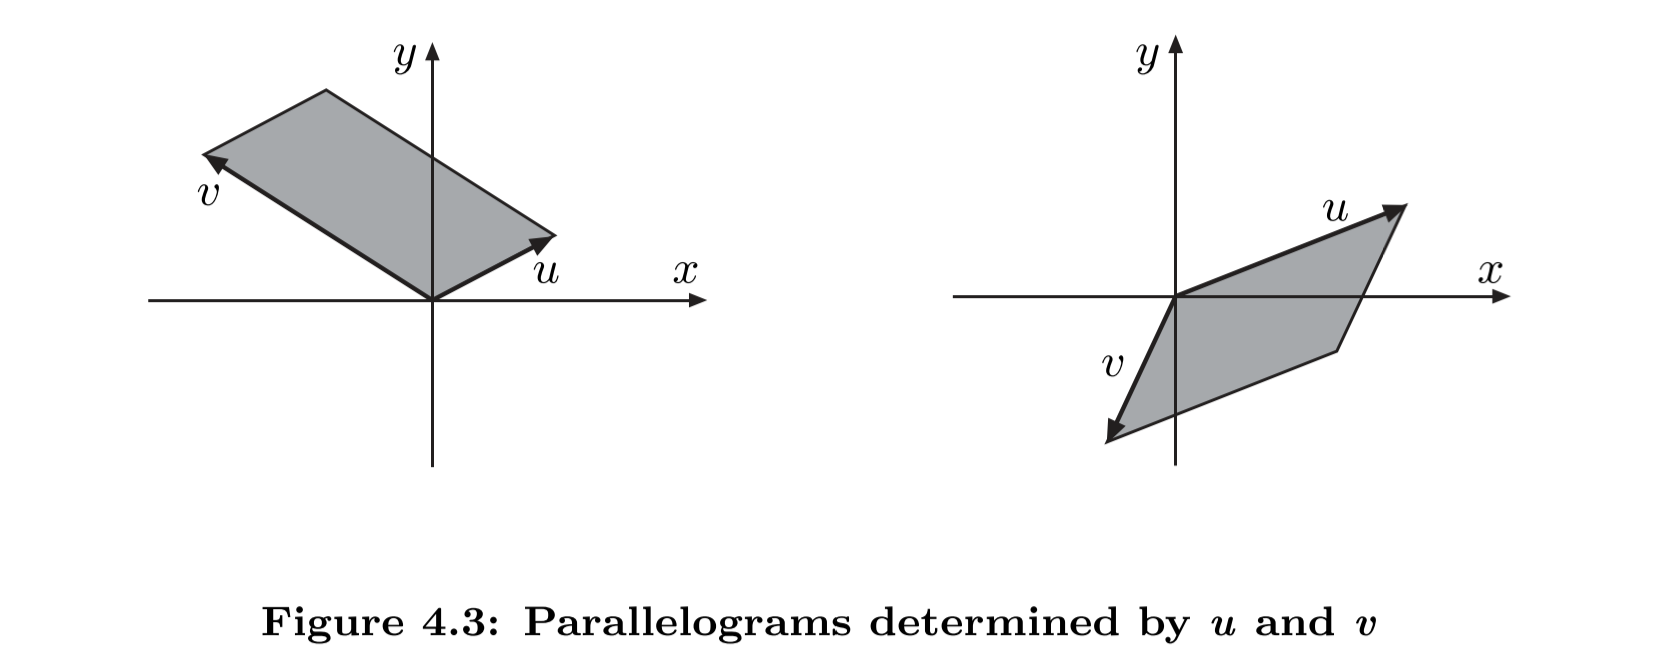
\includegraphics[width=16cm]{images/figure-4-3.png}

\begin{remark} \label{remark 4.1.4}
Observe that if the set \(\{ u, v \}\) is linearly \textbf{dependent} (i.e., if \(u\) and \(v\) are \emph{parallel}),
then the ``parallelogram'' determined by \(u\) and \(v\) is \emph{actually a line segment}, which we consider to be a
\href{https://www.wikiwand.com/en/Degeneracy_(mathematics)}{\textbf{degenerate}} parallelogram having area zero.
\end{remark}

\begin{additional theorem} \label{athm 4.1}
We have
\[
    \mathcal{A}\begin{pmatrix} u \\ v \end{pmatrix}
    = \left| \det \begin{pmatrix} u \\ v \end{pmatrix} \right|.
\]
Where \(\mathcal{A}\begin{pmatrix} u \\ v \end{pmatrix}\) denotes the area of the parallelogram determined by \(u\) and \(v\).
The proof is in the long and messy discussion below.
\end{additional theorem}

\begin{proof}
Since
\[
    \det \begin{pmatrix} u \\ v \end{pmatrix}
\]
may be negative, we cannot expect that
\[
    \mathcal{A}\begin{pmatrix} u \\ v \end{pmatrix} = \det \begin{pmatrix} u \\ v \end{pmatrix}.
\]
But \textbf{we can prove that}
\begin{equation} \label{area.formula}
    \mathcal{A}\begin{pmatrix} u \\ v \end{pmatrix} = \mathcal{O}\begin{pmatrix} u \\ v \end{pmatrix} \cdot \det \begin{pmatrix} u \\ v \end{pmatrix}
\end{equation}
from which it clearly follows that
\begin{equation} \label{simplified.area.formula}
    \mathcal{A}\begin{pmatrix} u \\ v \end{pmatrix} = \left| \det \begin{pmatrix} u \\ v \end{pmatrix} \right|.
\end{equation}
Our argument that \ref{area.formula} is correct employs a technique that, although somewhat indirect, can be \emph{generalized to \(\SET{R}^n\)}.
(Hence we will employ a similar argument in \SEC{4.2} and \SEC{4.3}.)

First, since
\[
    \mathcal{O} \begin{pmatrix} u \\ v \end{pmatrix} = \pm 1,
\]
we may multiply both sides of \ref{area.formula} by
\[
    \mathcal{O} \begin{pmatrix} u \\ v \end{pmatrix}
\]
to obtain the equivalent form
\[
    \mathcal{O}\begin{pmatrix} u \\ v \end{pmatrix} \mathcal{A}\begin{pmatrix} u \\ v \end{pmatrix} = \left(\mathcal{O}\begin{pmatrix} u \\ v \end{pmatrix}\right)^2 \cdot \det \begin{pmatrix} u \\ v \end{pmatrix} =
    1 \cdot \det \begin{pmatrix} u \\ v \end{pmatrix} =
    \det \begin{pmatrix} u \\ v \end{pmatrix},
\]
that is,
\begin{equation} \label{equivalent.area.formula}
    \det \begin{pmatrix} u \\ v \end{pmatrix}
    = \mathcal{O}\begin{pmatrix} u \\ v \end{pmatrix} \mathcal{A}\begin{pmatrix} u \\ v \end{pmatrix}.
\end{equation}
Hence \ref{equivalent.area.formula} is true if and only if \ref{area.formula} is true.
So we prove \ref{equivalent.area.formula} instead.

But first we \textbf{define} the function
\begin{equation} \label{def.delta}
    \delta \begin{pmatrix} u \\ v \end{pmatrix}
    = \mathcal{O}\begin{pmatrix} u \\ v \end{pmatrix}
      \cdot \mathcal{A}\begin{pmatrix} u \\ v \end{pmatrix}.
\end{equation}
And we will verify that \ref{def.delta} satisfies the three conditions of \EXEC{4.1.11}, and hence by \EXEC{4.1.11}, \(\delta\) is actually equal to \(\det\);
that is, \ref{equivalent.area.formula} is correct. (hence \ref{area.formula} is correct.)

\begin{note}
I recommend read \EXEC{4.1.11} first and go back to this very long and messy proof.
\end{note}

So we prove that \(\delta\) satisfies the three conditions in \EXEC{4.1.11} below:
\begin{enumerate}
\item For the first condition in \EXEC{4.1.11}, we need to show the four equations(given appropriate \(u, v, u_1, u_2, v_1, v_2, c\)):
\begin{align*}
    \delta \begin{pmatrix} u \\ cv \end{pmatrix}
    & = c \cdot \delta \begin{pmatrix} u \\ v \end{pmatrix} \\
    \delta \begin{pmatrix} cu \\ v \end{pmatrix}
    & = c \cdot \delta \begin{pmatrix} u \\ v \end{pmatrix} \\
    \delta \begin{pmatrix} u \\ v_1 + v_2 \end{pmatrix}
    & = \delta \begin{pmatrix} u \\ v_1 \end{pmatrix}
      + \delta \begin{pmatrix} u \\ v_2 \end{pmatrix} \\
    \delta \begin{pmatrix} u_1 + u_2 \\ v \end{pmatrix}
    & = \delta \begin{pmatrix} u_1 \\ v \end{pmatrix}
      + \delta \begin{pmatrix} u_2 \\ v \end{pmatrix}
\end{align*}
We begin by showing that for any real number \(c\)
\[
    \delta \begin{pmatrix} u \\ cv \end{pmatrix}
    = c \cdot \delta \begin{pmatrix} u \\ v \end{pmatrix}.
\]
Observe that this equation is valid if \(c = 0\) because
\begin{align*}
    \delta \begin{pmatrix} u \\ cv \end{pmatrix}
        & = \delta \begin{pmatrix} u \\ 0 \end{pmatrix} & \text{of course} \\
        & = \mathcal{O}\begin{pmatrix} u \\ 0 \end{pmatrix} \cdot \mathcal{A}\begin{pmatrix} u \\ v \end{pmatrix} & \text{by def in \ref{def.delta}} \\
        & = 1 \cdot \mathcal{A}\begin{pmatrix} u \\ v \end{pmatrix} & \text{by \RMK{4.1.3}} \\
        & = 1 \cdot 0 & \text{by \RMK{4.1.4}} \\
        & = 0 & \text{of course} \\
        & = 0 \cdot \delta \begin{pmatrix} u \\ v \end{pmatrix} & \text{of course} \\
        & = c \cdot \delta \begin{pmatrix} u \\ v \end{pmatrix}.
\end{align*}
So assume that \(c \ne 0\).
Regarding \(cv\) as the \emph{base of the parallelogram} determined by \(u\) and \(cv\), (by geometry formula) we see that
\begin{align*}
    \mathcal{A}\begin{pmatrix}
        u \\ cv
    \end{pmatrix}
    & = \text{(base of \(cv\) and \(u\))} \X \text{(altitude of \(cv\) and \(u\))} & \text{by geometry formula} \\
    & = \abs{c} \cdot (\text{length of } v) \X (\text{altitude of \(cv\) and \(u\)}) \\
    & = \abs{c} \cdot (\text{length of } v) \X (\text{altitude \textbf{of \(v\) and \(u\)}}) \\
    & \text{\ \ \ \ \ \ (since the altitude of these parallelograms are)} \\
    & \text{\ \ \ \ \ \ (the same; see Figure 4.4.)} \\
    & = \abs{c} \mathcal{A}\begin{pmatrix}
        u \\ v
    \end{pmatrix}. & \text{by geometry formula}
\end{align*}
So we have
\[
    \mathcal{A}\begin{pmatrix}
        u \\ cv
    \end{pmatrix}
    = \abs{c} \mathcal{A}\begin{pmatrix}
        u \\ v
    \end{pmatrix}. \text{ -- \MAROON{(a.1)}}
\]

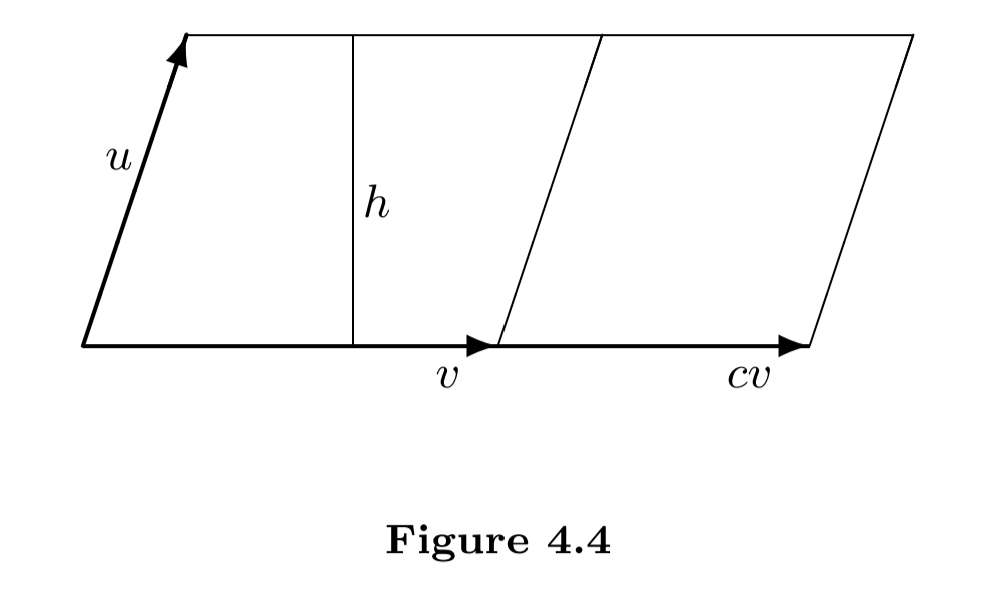
\includegraphics[width=10cm]{images/figure-4-4.png}

Hence
\begin{align*}
    \delta \begin{pmatrix}
        u \\ cv
    \end{pmatrix}
    & = \mathcal{O}\begin{pmatrix} u \\ cv \end{pmatrix} \cdot \mathcal{A}\begin{pmatrix} u \\ cv \end{pmatrix} & \text{by def in \ref{def.delta}} \\
    & = \left[\frac{c}{\abs{c}} \mathcal{O}\begin{pmatrix} u \\ v \end{pmatrix}\right] \mathcal{A}\begin{pmatrix} u \\ cv \end{pmatrix} & \text{need to prove but trivial by def of \(\mathcal{O}\)} \\
    & = \left[\frac{c}{\abs{c}} \mathcal{O}\begin{pmatrix} u \\ v \end{pmatrix}\right] \left[\abs{c} \mathcal{A}\begin{pmatrix} u \\ v \end{pmatrix}\right] & \text{by \MAROON{(a.1)}} \\
    & = c \cdot \mathcal{O}\begin{pmatrix} u \\ v \end{pmatrix} \cdot \mathcal{A}\begin{pmatrix} u \\ v \end{pmatrix} & \text{of course} \\
    & = c \cdot \delta \begin{pmatrix}
        u \\ v
    \end{pmatrix}. & \text{by def in \ref{def.delta}}
\end{align*}
A similar argument shows
\[
    \delta \begin{pmatrix}
        cu \\ v
    \end{pmatrix}
    = c \cdot \delta \begin{pmatrix}
        u \\ v
    \end{pmatrix}.
\]

So currently we have shown that
\[
    \delta \begin{pmatrix}
        u \\ cv
    \end{pmatrix}
    = c \cdot \delta \begin{pmatrix}
        u \\ v
    \end{pmatrix}.
    \text{ and }
    \delta \begin{pmatrix}
        cu \\ v
    \end{pmatrix}
    = c \cdot \delta \begin{pmatrix}
        u \\ v
    \end{pmatrix}. \text{ -- \BLUE{(1)}}
\]

Now before we prove the remaining two equations, we first prove that
\[
    \delta \begin{pmatrix}
        u \\ a\RED{u} + bw
    \end{pmatrix}
    = b \cdot \delta \begin{pmatrix}
        u \\ w
    \end{pmatrix}
\]
for any \(u, w \in \SET{R}^2\).
Because the parallelograms determined by \(u\) and \(w\) and by \(u\) and \(u + w\) \emph{have a common base} \(u\) and the same altitude (see Figure 4.5), (by geometry) it follows that
\[
    \mathcal{A} \begin{pmatrix}
        u \\ w
    \end{pmatrix}
    = \mathcal{A} \begin{pmatrix}
        u \\ \RED{u} + w
    \end{pmatrix}
\]
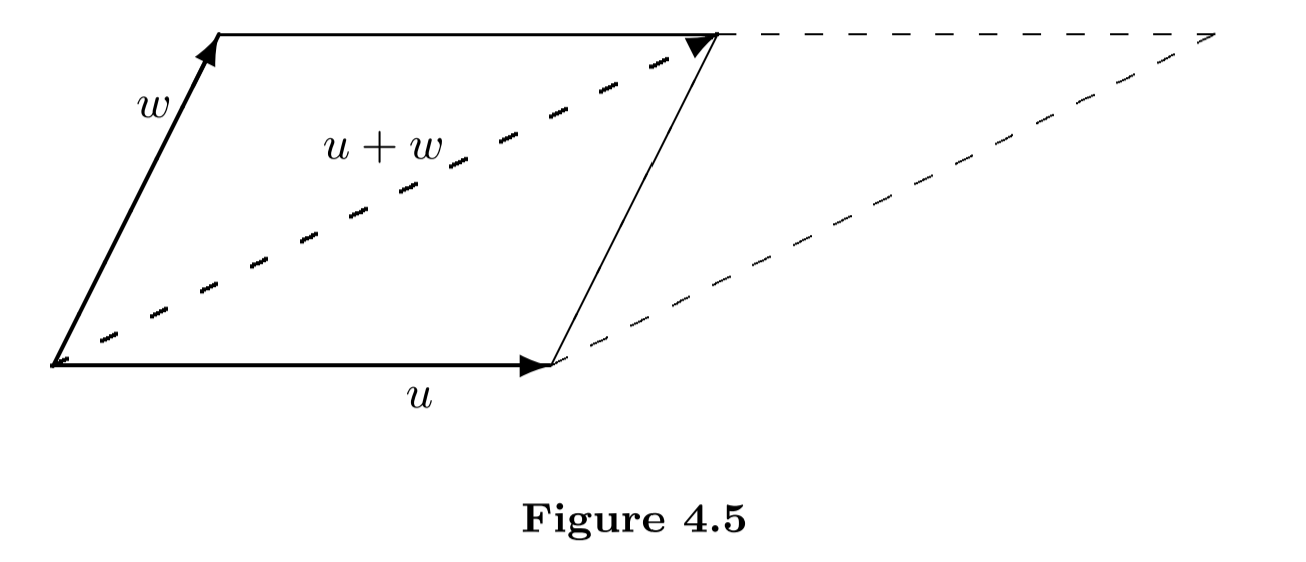
\includegraphics[width=14cm]{images/figure-4-5.png}

If \(a = 0\), then
\begin{align*}
    \delta \begin{pmatrix} u \\ au + bw \end{pmatrix}
    = \delta \begin{pmatrix} u \\ 0 + bw \end{pmatrix}
    & = \delta \begin{pmatrix} u \\ bw \end{pmatrix} \\
    & = b \cdot \delta \begin{pmatrix} u \\ w \end{pmatrix}. & \text{by \BLUE{(1)}}
\end{align*}
Otherwise, if \(a \ne 0\), then
\begin{align*}
    \delta \begin{pmatrix}
        u \\ au + bw
    \end{pmatrix}
    & = \delta \begin{pmatrix}
        u \\ a(u + \frac{b}{a}w)
    \end{pmatrix} & \text{of course} \\
    & = a \cdot \delta \begin{pmatrix}
        u \\ u + \frac{b}{a}w
    \end{pmatrix} & \text{by \BLUE{(1)}} \\
    & = a \cdot \delta \begin{pmatrix}
        u \\ \frac{b}{a}w
    \end{pmatrix} & \text{(indirectly) by Figure 4.5} \\
    & = a \left( \frac{b}{a} \right) \cdot \delta \begin{pmatrix}
        u \\ w
    \end{pmatrix} & \text{by \BLUE{(1)} again} \\
    & = b \cdot \delta \begin{pmatrix}
        u \\ w
    \end{pmatrix} & \text{of course}.
\end{align*}
So in all cases, we have
\[
    \delta \begin{pmatrix}
        u \\ au + bw
    \end{pmatrix}
    = b \cdot \delta \begin{pmatrix}
        u \\ w
    \end{pmatrix}. \text{ -- \BLUE{(2)}}
\]
Finally, we now are able to show that
\[
    \delta \begin{pmatrix}
        u \\ v_1 + v_2
    \end{pmatrix}
    = \delta \begin{pmatrix}
        u \\ v_1
    \end{pmatrix}
    + \delta \begin{pmatrix}
        u \\ v_2
    \end{pmatrix}
\]
for all \(u, v_1, v_2 \in \SET{R}^2\).
Since the result is immediate if \(u = 0\)
(that will cause every term to be zero, since the area of the corresponding parallelogram will we zero),
we assume that \(u \ne 0\).
Choose any vector \(w \in \SET{R}^2\) such that \(\{ u, w \}\) is \emph{\LID{}}.
Then for any vectors \(v_1, v_2 \in \SET{R}^2\) there exist (unique) scalars \(a_i\) and \(b_i\) such that
\[
    v_i = a_i u + b_i w \ \  (i = 1, 2). \text{ -- \MAROON{(a.2)}}
\]
Thus
\begin{align*}
    \delta \begin{pmatrix}
        u \\ v_1 + v_2
    \end{pmatrix}
    & = \delta \begin{pmatrix}
            u \\ (a_1 + a_2) \RED{u} + (b_1 + b_2) w
        \end{pmatrix} & \text{by \MAROON{(a.2)}} \\
    & = (b_1 + b_2) \delta \begin{pmatrix}
            u \\ w
        \end{pmatrix} & \text{by \BLUE{(2)}} \\
    & = b_1 \delta \begin{pmatrix}
            u \\ w
        \end{pmatrix}
      + b_2 \delta \begin{pmatrix}
            u \\ w
        \end{pmatrix} & \text{of course} \\
    & = \delta \begin{pmatrix}
            u \\ a_1 u + b_1 w
        \end{pmatrix}
      + \delta \begin{pmatrix}
            u \\ a_2 u + b_2 w
        \end{pmatrix} & \text{again by \BLUE{(2)}} \\
    & = \delta \begin{pmatrix}
            u \\ v_1
        \end{pmatrix}
      + \delta \begin{pmatrix}
            u \\ v_2
        \end{pmatrix} & \text{by \MAROON{(a.2)}}
\end{align*}
A similar argument shows that
\[
    \delta \begin{pmatrix}
        u_1 + u_2 \\ v
    \end{pmatrix}
    = \delta \begin{pmatrix}
            u_1 \\ v
        \end{pmatrix}
      + \delta \begin{pmatrix}
            u_2 \\ v
        \end{pmatrix}
\]
for all \(u_1, u_2, v \in \SET{R}^2\).

So finally, we have proved that the four equations in the first condition of \EXEC{4.1.11} are satisfied by definition of \(\delta\) in \ref{def.delta}.

\item
Since (by geometry) \(\mathcal{A} \begin{pmatrix} u \\ u \end{pmatrix} = 0\), it follows that
\begin{align*}
    \delta \begin{pmatrix} u \\ u \end{pmatrix}
    & = \mathcal{O} \begin{pmatrix} u \\ u \end{pmatrix} \cdot \mathcal{A} \begin{pmatrix} u \\ u \end{pmatrix} & \text{by def in \ref{def.delta}} \\
    & = 0
\end{align*}
for any \(u \in \SET{R}^2\).

\item
Because (by geometry) the parallelogram determined by \(e_1\) and \(e_2\) is the \emph{unit square},
\begin{align*}
    \delta(I_2)
    & = \delta \begin{pmatrix} e_1 \\ e_2 \end{pmatrix} \\
    & = \mathcal{O} \begin{pmatrix} e_1 \\ e_2 \end{pmatrix} \cdot \mathcal{A} \begin{pmatrix} e_1 \\ e_2 \end{pmatrix} & \text{by def in \ref{def.delta}} \\
    & = 1 \cdot \mathcal{A} \begin{pmatrix} e_1 \\ e_2 \end{pmatrix} & \text{of course (by calculation)} \\
    & = 1 \cdot 1 & \text{since the parallelogram is the unit square} \\
    & = 1.
\end{align*}
\end{enumerate}

Therefore, \(\delta\) defined in \ref{def.delta} satisfies the three conditions of \EXEC{4.1.11}, and hence \(\delta = \det\).
Hence \ref{equivalent.area.formula}, \ref{area.formula} and \ref{simplified.area.formula} are correct;
that is,
\[
    \mathcal{A}\begin{pmatrix} u \\ v \end{pmatrix}
    = \mathcal{O}\begin{pmatrix} u \\ v \end{pmatrix} \cdot \det \begin{pmatrix} u \\ v \end{pmatrix}
    = \left| \det \begin{pmatrix} u \\ v \end{pmatrix} \right|.
\]
\end{proof}

Thus we see, for example, that the area of the parallelogram determined by \(u = (-1, 5)\) and \(v = (4, -2)\) is
\[
    \left| \det \begin{pmatrix}
        u \\ v
    \end{pmatrix} \right|
    = \left| \det \begin{pmatrix}
        -1 & 5 \\ 4 & -2
    \end{pmatrix} \right|
    = 18.
\]
